\documentclass{article}
\usepackage{graphicx}
\usepackage{fontspec}
\setmainfont{Arial}
\setlength{\parindent}{0pt}
\begin{document}
\section{Users can save money}

Situation now:
\begin{itemize}
\item translate a document to 10 languages
\item each translation costs 1.000€
\item \textbf{cost: 10.000€}
\end{itemize}

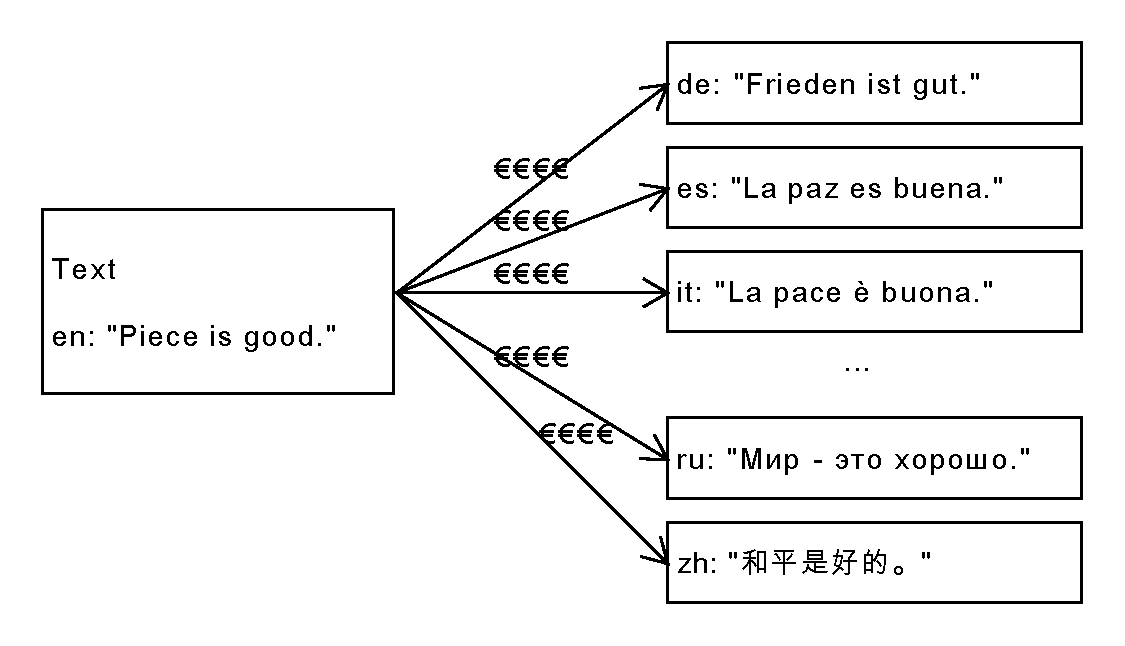
\includegraphics[scale=0.4]{dia/user-view-current-world.pdf}

Goal:
\begin{itemize}
\item encode the document
\item generate 10 language versions
\item encoding costs 2.000€
\item generation doesn't cost anything
\item \textbf{cost: 2.000€}
\end{itemize}

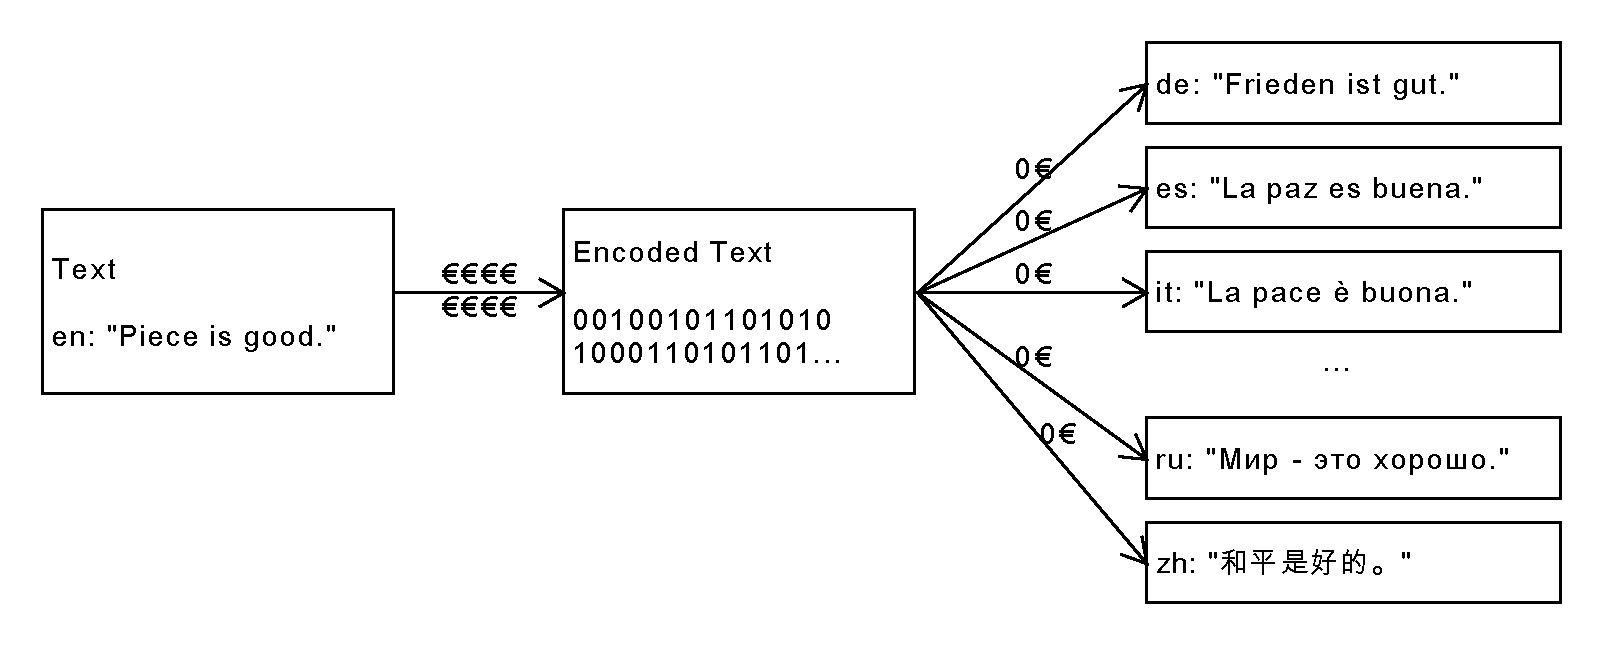
\includegraphics[scale=0.4]{dia/user-view-tokimani.pdf}

Saving: \textbf{8.000€}

\subsection{Some facts about costs}
TODO: how much is spent on translation in the year 2019

TODO: 1.000€ is the cost to translate a document of: 

TODO: in Branchenkennz: xx precent translate to more than k languages.

\end{document}
